\documentclass[dvipdfmx]{jsarticle}

\title{JavaScript入門その1}
\author{原著者:清水健二 / 改訂:糠山誠一}
\date{2020-06-13}
\usepackage{tcolorbox}
\usepackage{color}
\usepackage{listings, plistings}

% Java
\lstset{% 
  frame=single,
  backgroundcolor={\color[gray]{.9}},
  stringstyle={\ttfamily \color[rgb]{0,0,1}},
  commentstyle={\itshape \color[cmyk]{1,0,1,0}},
  identifierstyle={\ttfamily}, 
  keywordstyle={\ttfamily \color[cmyk]{0,1,0,0}},
  basicstyle={\ttfamily},
  breaklines=true,
  xleftmargin=0zw,
  xrightmargin=0zw,
  framerule=.2pt,
  columns=[l]{fullflexible},
  numbers=left,
  stepnumber=1,
  numberstyle={\scriptsize},
  numbersep=1em,
  language={Java},
  lineskip=-0.5zw,
  morecomment={[s][{\color[cmyk]{1,0,0,0}}]{/**}{*/}},
}
%\usepackage[dvipdfmx]{graphicx}
\usepackage{url}
\usepackage[dvipdfmx]{hyperref}
\usepackage{amsmath, amssymb}
\usepackage{itembkbx}
\usepackage{eclbkbox}	% required for `\breakbox' (yatex added)
\fboxrule=0.5pt
\parindent=1em
\begin{document}

%% 修正時刻: Sat Jun 13 16:00:25 2020


\section{DOMを操作する}

ブラウザの画面に表示するために \verb!document.write(`<li>${listText}</li>`)! などと
していましたが、document.write は その挙動の不安定さからHTML5 では \textbf{非推奨}
となっています。

では、ブラウザの画面上に文字を出力したり、\verb!<h1>! などのタグを出力したりするには
どうするかというと、タグやid、class で構成された要素を取得し、その取得した要素に対して
さまざまな文字を追加したり、\verb!<li>!などのタグを追加したりします。

ブラウザは文章や画像などのコンテンツとHTMLの構造からなるオブジェクトで、その表現形態を
\textbf{DOM} (Document Object Model) といいます。

\textbf{DOM} は、HTMLのための「プログラミングインターフェース」と言えます。
言い換えるなら、ウェブページを「表現、保存、操作する方法」と言えます。
\footnote[1]{「DOMの紹介」  \url{https://developer.mozilla.org/ja/docs/Web/API/Document\_Object\_Model/Introduction}}

\subsubsection{DOMにアクセスしてブラウザの表示を変える}

start.htmlの\verb!<body>!の中に画像を表示している部分があります。
その部分に以下のように onclick属性をつけます。

\fbox{ \textless img id=''img1'' src=''images/4.jpg'' alt='''' onclick=''kansu3();'' \textgreater}

onclick属性をつけたことで、この画像をクリックすると ''kansu3'' という関数が実行されることになります。

\footnote[2]{ onclick -- HTMLのタグの中に JavaScript の記述を入れることを嫌がる人もいます。HTMLを汚すからというわけです。たしかにここで onclick を使わなくても JavaScriptの文中でクリックイベントを検知するやり方はいくつかあります。このあたりはポリシーの問題だと思います。もっとも、onclick の記述が必要な箇所が多数あるのであれば、いちいち onclick を記述せずとも、JavaScript文中で他の方法を使ったほうが楽だし、間違いも少くてすみます。}

さて、この kansu3という関数をどこに書くかですが、\verb!</body>! タグの直前の \verb!<script>...</script> 内に記述します。これは、\verb!<img>! などのbody要素の中身すべてを読み込んだあとに記述するという意味があります。これは、JavaScript文中で bodyの中のタグ名、id名、class名などを使用するということです。

以下のように kansu3 の内容を書いてください。

\begin{lstlisting}
 <script>
   function kansu3 () {
     document.getElementById('heading1').textContent = 'Change!';
   }
 </script>
\end{lstlisting}

画像をクリックすると \verb!<h1>!要素が「Change!」に変わります。\fbox{.textContent} は、その要素の文字列を書き換えるメソッドです。\\
今度は 'Change!' を \verb|'<i>Change!</i>'| としてみてください。\\

\fbox{ 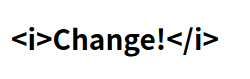
\includegraphics[width=5cm]{change.png}}

\fbox{.textContent} は、タグも含めてそのまま文字列として出力します。\\
タグを有効にして要素の中身にHTML要素をつけ加えるには \fbox{.innerHTML} を使います。
\footnote[1]{ほかに .insertAdjacentHTML というメソッドもあります。これは要素をつけ加える際に
つけ加える位置を指定できます。.innerHTML よりも強力です。}

\begin{lstlisting}
 <script>
   function kansu3 () {
     document.getElementById('heading1').innerHTML = '<i>Change!</i>';
   }
 </script>
\end{lstlisting}

今度は画像ファイルを変更します。src属性を書き換えるのです。\\
kansu3 の内容を以下のように変更してください。

\begin{lstlisting}
 <script>
   function kansu3 () {
     document.getElementById('img1').src = 'images/2.jpg';
   }
 </script>
\end{lstlisting}

画像をクリックすると画像が切り変わりました。\\
document.getElementById は、複数指定できます。

\begin{lstlisting}
 <script>
   function kansu3 () {
     document.getElementById('img1').src = 'images/2.jpg';
     document.getElementById('img1').style.width = '400px';
   }
 </script>
\end{lstlisting}

\fbox{.getElementById} は Webページ内の id で指定された要素を取得するメソッドです。\\
class で指定された要素を取得するには \fbox{.getElementsByClassName} を使います。また、
\verb!<img>! などのタグ名で要素を取得するには \fbox{.getElementsByTagName} を使います。
ただ両方とも取得できるのは要素ではなく、\textbf{コレクション} という複数の要素の固まりです。
これの扱いはもう少し経ってからのほうがいいです。

\subsection{変数によるオブジェクトの取得}

先ほどは .getElementById を2回使って画像の src属性とstyle属性を書き換えていましたが、
変数を使うと効率よく行えます。\\
さっきの kansu3 の記述を以下のようにします。

\begin{lstlisting}
 <script>
   function kansu3 () {
     const eleImage = document.getElementById('img1');
     eleImage.src = 'images/2.jpg';
     eleImage.style.width = '400px';
   }
 </script>
\end{lstlisting}

''img1'' というid名をもつ \verb!<img>! 要素を取得し、eleImage という名前の変数を作ってそれに
 格納しています。\footnote[1]{このようなブラウザを構成している要素のことを \textbf{オブジェクト} といいます。
 この eleImage がどのようなものかは \fbox{ console.log(eleImage); } としてみるとわかります。}
 あるいは、.getElementById で取得したものに 「eleImage という名前をつけた」と考えてもいいと思います。
 そうすることで、あとの処理が簡単になります。

 変数をうまく使うと以下のようなこともできます。kansu3 の記述を以下のように書き換えてください。

\begin{lstlisting}
 <script>
   let imageSize = 0;
   function kansu3 () {
     const eleImage = document.getElementById('img1');
     imageSize += 5; 
     eleImage.style.width = 200 + imageSize + 'px';
   }
 </script>
\end{lstlisting}
 
 \fbox{ += 5 } というのは、「+5 して代入」という意味です。画像をクリックするたびに画像が 5pxずつ
 大きくなります。

 \subsection{setIntervalで非同期処理}
 \footnote[2]{非同期処理とは、複数の処理をおこなう際に、一つの処理の完了を待たずに次の処理をおこなうことです。その時、一つの処理が終了したときに次の処理を登録しておきます。日常生活での非同期処理の代表的なものに料理があります。御飯が炊き上がるまでに他の調理をしますし、おみそ汁を作りながら魚を包丁で切ったりします。}

 先ほどはクリックするたびに画像が大きくなりましたが、今度は時間の経過とともに自動的に大きくします。
 ただ、いつまでも大きくなっていくと困るので、幅400pxの大きさになればストップします。

\begin{lstlisting}
 <script>
   let imageSize = 0;
   const intervalId = setInterval( kansu3, 100 );        --- <1>
   const eleImage = document.getElementById('img1');     --- <2>
 
   function kansu3 () {
     imageSize += 5; 
     eleImage.style.width = 200 + imageSize + 'px';
     if (imageSize > 200) {
       clearInterval( intervalId );                        --- <3>
     }
    }
 </script>
\end{lstlisting}
 
 \begin{itemize}
  \item [\textless 1\textgreater] setIntervalは、100ミリ秒(10分の1秒)ごとに kansu3 を実行します。
        そして自己の実行プロセスのナンバーを intervalId にセットしています。
  \item [\textless 2\textgreater] 今までは kansu3 が呼び出される度に getElementById で \verb!<img>!
        を取得していましたが、kansu3 の外に移動することで、最初に取得して変数eleImage に入れて
        おけば、kansu3 の中では eleImage に対して処理を行なえばいいことになります。
  \item [\textless 3\textgreater] 200 + imageSize が400を超えると、clearIntervalの処理がおこなわれ
        ます。clearInterval は setInterval の処理をストップします。その際に、setIntervalを設定
        したときのid すなわち intervalId を指定します。
 \end{itemize}

 \subsection{日付オブジェクトを使う}

 JavaScriptで日付を管理するには Date オブジェクトを利用します。
 kansu3 を記述していた部分を以下のように書き換えてください。

 \begin{lstlisting}
  <script>
    const hiduke = new Date();
    const timeText = document.getElementById('heading1');
    timeText.insertAdjacentHTML('afterend', `<time>${hiduke}</time>`);
  </script>
 \end{lstlisting}

 
 
\end{document}

%% 修正時刻: Sat May  2 15:10:04 2020


%% 修正時刻: Sun Jun 14 13:40:02 2020
